\documentclass{patmorin}
\usepackage{amsthm,amsmath,graphicx,stmaryrd}
\usepackage{pat}


\DeclareMathOperator{\asf}{asf}
\DeclareMathOperator{\depth}{depth}

\title{\MakeUppercase{Good Average Stretch Geometric Spanners}}
\author{Vida Dujmovi\'c, Pat Morin, and Michiel Smid}


\begin{document}
\begin{titlepage}
\maketitle

\begin{abstract}
  We show that, for any set $V$ of $n$ points in $\R^d$, there exists
  a geometric graph with vertex set $V$, $O(n)$ edges, and that has
  average stretch factor $1+ O((\log n/n)^{1/2d})$.
  We also show that, even in $\R^2$, there exists point sets for which
  any graph with a linear number of edges has average stretch factor
  at least $1+\Omega(1/\sqrt{n})$.
\end{abstract}

\end{titlepage}

\section{Introduction}

The \emph{average stretch factor} of a geometric graph, $G$, with vertex
set $V(G)\subset \R^d$ and edge set $E(G)$ is
\[
    \asf(G) = \binom{|V(G)|}{2}^{-1}\sum_{\{u,w\}\in\binom{V(G)}{2}}\frac{\|uw\|_G}{\|uw\|}
\]
where $\|uw\|$ denotes the Euclidean distance between $u$ and $w$
and $\|uw\|_G$ denotes the shortest Euclidean path from $u$ to $w$
that uses only edges of $G$.

In this paper we show that, for any constant dimension, $d$, and any
finite set $V\subset \R^d$, there exists a geometric graph $G=(V,E)$
having $|E|=O(n)$ edges and such that $\asf(G)=1+o_n(1)$.

\section{The Construction}

The construction of a good average stretch factor graph, $G=(V,E)$,
makes use of a clustering of the points of $V$ into $O(n/k)$ clusters of
size at most $k$ that we call a $k$-partition.  In the next subsection,
we define $k$-partitions and show how to compute them.  In the following
subsection we show how to construct the graph $G$.

\subsection{$k$-Partitions}

We make use of the following construct:  A \emph{$k$-partition} of a
set $V$ of $n$ points in $\R^d$ consists of a set, $D$, of balls and an
assignment $f:V\to D$ such that
\begin{enumerate}
  \item $|D|\in O(n/k)$,
  \item for each $u\in V$, $u\in f(u)$ (i.e., $u$ is a assigned to a
    ball that contains $u$),
  \item for each $\Delta\in D$, $|\{u\in V: f(u)=\Delta\}|\le k$ (i.e.,
   at most $k$ points are assigned to each ball),
  \item for every $r> 0$, $c\ge 2$, and $p\in\R^2$, the number of balls
   in $D$ whose radius is in the range $[r,2r)$ and that contain $p$
   is $O(1)$.
\end{enumerate}

Note that, aside from Property~4, there is very little structure to
the balls in $D$. In particular, balls in $D$ may overlap and may even
contain each other.

\begin{lem}
  For any set $V$ of $n$ points, a $k$-partition of $V$ exists and can
  be found in $O(n\log n)$ time.
\end{lem}

\begin{proof}
  We construct a $k$-partition using the binary \emph{fair-split
  tree}, $T=T(V)$, which is defined recursively as follows
  \cite{callahan.kosaraju:decomposition}: If $V$ consists of a single
  point, $u$, then $T$ contains a single node corresponding to $u$.
  Otherwise, consider the minimal axis-aligned bounding box, $B(V)$,
  that contains $V$.  The root of $T$ corresponds to $B(V)$ and this
  box is split into two boxes $B_1(V)$ and $B_2(V)$ by cutting $B(V)$
  with a hyperplane in the middle of its longest side.  The left and
  right subtrees of the root are defined recursively by constructing
  fair-split trees for $B_1(V)\cap V$ and $B_2(V)\cap V$. See \figref{fst}.

  \begin{figure}
    \begin{center}
      \includegraphics{whole-thing}
    \end{center}
    \caption{A fair split tree for $V$ repeatedly by splits the bounding
      box $B(V)$ in the middle of its longest side.}
    \figlabel{fst}
  \end{figure}

  For each node, $u$, of $T$ there is a naturally defined subset
  $V(u)\subseteq V$ of points associated with $u$ as well as a bounding
  box $B(u)=B(V(u))$.  Since $T$ is a binary tree with $2n+1$ nodes, it
  has a set of $t-1$ edges whose removal partitions the vertices of $T$
  into $t\in O(n/k)$ maximally-connected components $C_1,\ldots,C_t$,
  each having at most $k$ vertices.

  For each $i\in\{1,\ldots,t\}$, let $u_i$ denote the root of the
  subtree $C_i$.  To obtain the balls, $\Delta_1,\ldots,\Delta_t$, of
  the $k$-partition we take, for each $i\in\{1,\ldots,t\}$ the smallest
  ball, $\Delta_i$ that contains $B(u_i)$.  For the mapping $f$, we
  map the point associated with each leaf, $w$, of $T$ to the unique
  ball $\Delta_i$, where $C_i$ contains $w$.  (Note that some balls,
  $\Delta_i$, may have no points mapped to them if $C_i$ contains no
  leaves of $T$; see \figref{fst-2}.)

  \begin{figure}
    \begin{center}
      \includegraphics{whole-thing2}
    \end{center}
    \caption{The fair split tree is partitioned into subtrees of size
    $k$ (${}=3$) by removing $O(n/k)$ edges.  The root, $u_i$, of each subtree
    defines a ball, $\Delta_i$, in the $k$-partition. (The ball $\Delta_1$
    is omitted from this figure.)}
    \figlabel{fst-2}
  \end{figure}


  The fair-split tree, $T$, and the boxes, $B(u)$, associated
  with each node, $u$, of $T$ can be computed in $O(n\log n)$ time
  \cite{callahan.kosaraju:decomposition}.  The partition of the vertices
  of $T$ into components $C_1,\ldots,C_t$ can easily be done in $O(n\log
  n)$ time by repeatedly finding an edge of a component of size $k'>k$
  that partitions that component into two pieces each of size at most
  $\lceil 2k'/3\rceil$.  Thus, the construction of $D$ and $f$ can be
  accomplished in $O(n\log n)$ time.

  The set of balls $D=\{\Delta_1,\ldots,\Delta_t\}$ and the
  mapping $f:V\to D$ described in the preceding paragraphs clearly
  satisfy Properties~1--3 in the definition of a $k$-partition.
  What remains is to show that they also satisfy Property~4. For a
  node $u$ in $T$, let $L(u)$ denote the length of the longest side
  of $B(u)$.  We make use of the following result on fair split trees
  \cite[Lemma~9.4.3]{narasimhan.smid:geometric}:

  \begin{lem}\lemlabel{box-packing}
     Let $C$ be a box whose longest side has length $\ell$ and let
     $\alpha >0$ be any positive real number.  Let $w_1,\ldots,w_s$
     be some nodes of a fair-split tree, $T$, such that
     \begin{enumerate}
       %\item $w_i$ is not the root of $T$, for all $i\in\{1,\ldots,s\}$;
       \item the sets $V(w_i)$ are disjoint, for all $i\in\{1,\ldots,s\}$;
       \item $L(w_i)\ge \ell/\alpha$, for all
          $i\in\{1,\ldots,s\}$;\footnote{The original lemma
          \cite[Lemma~9.4.3]{narasimhan.smid:geometric} is slightly
          stronger in that it only requires that $L(w_i')\ge \ell/\alpha$,
          where $w_i'$ is the parent of $w_i$.} and
       \item $B(w_i)$ intersects $C$, for all $i\in\{1,\ldots,s\}$.
     \end{enumerate}
     Then $s\le (2\alpha + 2)^d$.
  \end{lem}
  %Note that the first condition of \lemref{box-packing} is equivalent
  %to the statement that no $u_i$ is an ancestor of $u_j$ for any
  %$\{i,j\}\subseteq\{1,\ldots,k\}$, which also implies that the interiors of
  %$B(u_i)$ and $B(u_j)$ are disjoint.

  To prove that the balls in $D$ satisfy Property~4 of a $k$-partition,
  let $\{\Delta_{i_1},\ldots,\Delta_{i_q}\}\subseteq D$ be the subset of
  balls in $D$ having radii in the interval $[r,2r)$ and that all contain
  some common point, $p\in\R^d$.   Then each such ball, $\Delta_{i_j}$
  corresponds to a node $u_{i_j}$ of $T$ such that
  \begin{equation}
        \frac{r}{\sqrt{d}} \le L(r_{i_j}) \le 4r \enspace . \eqlabel{bounds}
  \end{equation}
  Therefore, each box $B(u_{i_j})$ intersects a ball of radius $2r$
  centered at $p$.  (Indeed, the center of $B(u_{i_j})$ is contained in
  this ball.)  Therefore, each box $B(u_{i_j})$ intersects a box, $C$, of
  side-length $4r$ centered at $p$.  

  We are almost ready to apply \lemref{box-packing} to
  $C$---whose side length is $\ell = 4r$---and the vertex set
  $w_1,\ldots,w_q=u_{i_1},\ldots,u_{i_q}$. For each $j\in\{1,\ldots,q\}$,
  $B(u_{i_j})$ intersects $C$, so Condition~3 of \lemref{box-packing}
  is satisfied.  Furthermore, \eqref{bounds} states that $L(u_{i_j})\ge
  r/\sqrt{d} = \ell/(4\sqrt{d})$, so Condition~2 of \lemref{box-packing}
  is satisfied with $\alpha=4\sqrt{d}$.  Unfortunately, there is still
  a little more work to do since the nodes $u_{i_1},\ldots,u_{i_t}$
  do not necessarily satisfy Condition~1 of \lemref{box-packing}.

  To proceed, we partition $u_{i_1},\ldots,u_{i_q}$ into a small number of
  subsets, each of which satisfies Condition~1 of \lemref{box-packing}.
  Observe that Condition~1 of \lemref{box-packing} is equivalent
  to the statement that no $w_i$ is an ancestor of $w_j$ for any
  $\{i,j\}\subseteq\{1,\ldots,s\}$.  A key observation is that, if $u$
  is an ancestor of $w$ in a fair-split tree, $T$, and the difference
  in depth between $u$ and $w$ is $d$, then
  \[
      L(u) \ge 2L(w) \enspace .
  \]
  This, and \eqref{bounds}, implies that, if $u_{i_j}$ is an ancestor
  of $u_{i_{j'}}$ then
  \[
     \depth(u_{i_{j'}})-\depth(u_{i_{j}}) \le d\log(4\sqrt{d}) \enspace .
  \]
  Thus, we can partition $u_{i_1},\ldots,u_{i_q}$ into $z=\lceil
  d\log(4\sqrt{d})\rceil$ subsets, $S_0,\ldots,S_{z-1}$, each of which
  satisfies Condition~1 of \lemref{box-packing}, by assigning $u_{i_j}$
  to the subset $S_{\depth(u_{i_j})\bmod z}$.  

  Now, \lemref{box-packing} implies that, for each $i\in\{0,\ldots,z-1\}$, 
  \[
     |S_i|\le (8\sqrt{d}+2)^d
  \]
  so that
  \[
     q = \sum_{i=0}^{z-1}|S_i|\le (8\sqrt{d}+2)^dz = (8\sqrt{d}+2)^d\lceil d\log(4\sqrt{d})\rceil  \in O(1) \enspace .
  \]
  Thus, for any point $p\in\R^d$, the set of balls in $D$ whose radius
  is in the interval $[r,2r)$ and that contain $p$ has size $O(1)$.
  Therefore the balls in $D=\Delta_1,\ldots,\Delta_t$ satisfy Property~4
  in the definition of a $k$-partition.  This completes the proof.
\end{proof}

\subsection{The Graph $G$}

With the availability of $k$-partitions, we are now ready to prove our
main result.

\begin{thm}\thmlabel{upper-bound}
  For every set constant dimension, $d$ and every set, $V$, of
  $n<\infty$ points in $\R^d$, there exists a geometric graph $G$ with
  $V(G)=V$, $|E(G)|\in O(n)$ and $\asf(G)=1+o_n(1)$.  More precisely,
  $\asf(G)=1+O((\log n/n)^{1/2d})$.
\end{thm}

\begin{proof}
  In the following proof, the variables $c,k\in\omega_n(1)$ and $\delta\in
  o_n(1)$ are used before they are specified.  Values of these variables
  that optimize the average spanning ratio are given at the end of
  the proof.

  We begin with a $k$-partition $(\{\Delta_1,\ldots,\Delta_{n'}\},f)$
  of $V$, and we use the convention that $\Delta_1,\ldots,\Delta_{n'}$
  are ordered by decreasing size.  For each $i\in \{1,\ldots,n'\}$,
  let $V_i=\{u\in V : f(u)=\Delta_i\}$; that is, $V_i$ is the set of
  points assigned to the ball $\Delta_i$.  For each set $V_i$, we choose a
  representative vertex, $u_i$, and add edges joining $u_i$ to each other
  vertex in $V_i$ (see \figref{overview}). Let $N=\{u_1,\ldots,u_{n'}\}$
  denote the set of representative vertices and recall that $|N|=n'\in
  O(n/k)$.

  \begin{figure}
    \begin{center} 
      \includegraphics{overview}
    \end{center} 
    \caption{Using a $k$-partition, $G$ contains $O(n/k)$ stars whose
      centers are interconnected by a $(1+1/k^{1/(d-1)})$-spanner}
    \figlabel{overview}
  \end{figure}

  Next, we add two spanner constructions to $G$.  The first is a
  $(1+1/k^{1/(d-1)})$-spanner of $N$ and the second is a $2$-spanner
  of $V$.  The first construction adds $O(k|N|)=O(n)$ edges to $G$
  \cite[Section~5.5]{narasimhan.smid:geometric}, while the second adds
  $O(n)$ edges \cite{x,ys,ss}.  With the addition of these extra edges
  we have, for any $u,w\in V$
  \[
     \frac{\|uw\|_G}{\|uw\|} \le \begin{cases}
           1+1/k^{1/(d-1)} & \text{if $u,w\in N$} \\
           2 & \text{in any case.}
         \end{cases}
  \]
  
  Let $r_i$ denote the radius of $\Delta_i$ and let $D_i$ be a ball
  centered at the center of $\Delta_i$ and having radius $cr_i$.
  Points of $V$ that are in $D_i\setminus \Delta_i$ can be problematic
  for $V_i$; there is no guarantee that such points have a $1+o(1)$
  spanning path to the points in $V_i$.  The final step in the spanner
  construction attempts to deal with most of these problematic points.

  For each $i\in\{1,\ldots,n'\}$, we find a ball, $E_i$, of radius
  $r_i/c$, with center in $D_i$, and that contains the maximum number
  of points of $V$.  (Note that this may include points of $V$ in $V_i$
  or outside of $D_i$.)  We then add edges joining each of the points
  in $V_i$ to some point in $E_i$.  See \figref{hitter}.

  \begin{figure}
    \begin{center}
      \includegraphics{hitter}
    \end{center}
    \caption{The ball $E_i$ captures as many points of $V$ as possible
     while still having center in $D_i$.}
    \figlabel{hitter}
  \end{figure}

  This concludes the description of the graph $G$.  In determining the
  average stretch factor of $G$, there are four types of pairs of points,
  $u\in V_i$, $w\in V_j$, $j\ge i$, to consider:
  \begin{enumerate}
    \item Pairs that are both from the same set; i.e., where $i=j$.  Each such
      pair has $\|uw\|_G/\|uw\|\le 2$ and each set $V_i$ contributes at
      most $\binom{k}{2}$ pairs to average, so their total contribution
      to the average is at most
      \[
        2\cdot\binom{n}{2}^{-1}\cdot\binom{k}{2}\cdot O(n/k) \in O(k/n)
        \enspace .
      \]
    \item Pairs for which $w$ is outside of $D_i$.  For each
      such pair, 
      \[
        \|uw\|_G/\|uw\|\le (1+1/k^{1/(d-1)})(1+O(1/c)) \in O(1+1/k^{1/(d-1)}+1/c) \enspace .
      \]
    \item Pairs for which $w$ is contained in $E_i$.  For each
      such pair, 
      \[
        \|uw\|_G/\|uw\|\le 1+O(1/c) \enspace .
      \]
    \item Pairs for which $w$ is contained in $D_i'$.  For each
      such pair, $\|uw\|_G/\|uw\|\le 2$.  The number of such pairs is no
      more than $k\sum_{i=1}^{n'}|V\cap D_i'|$, so the total contribution
      of such pairs to the average stretch factor is at most
      \[
            \binom{n}{2}^{-1}\cdot\left(k\sum_{i=1}^{n'} |V\cap D_i'|\right)\cdot 2 \enspace .
      \]
  \end{enumerate}

%  As we will see, the only problematic points that remain for $V_i$
%  are those contained in $D_i'=D_i\setminus E_i$.  The average stretch
%  factor of $G$ can be expressed as
%  \begin{align*}
%    \asf(G) 
%      & = 
%      \binom n2^{-1}\left(
%        \sum_{i=1}^{n'}\sum_{u,w\in V_i}\frac{\|uw\|_G}{\|uw\|}  
%         + \sum_{i=1}^{n'-1}\sum_{j={i+1}}^{n'}
%            \sum_{u\in V_i}\sum_{w\in V_j}\frac{\|uw\|_G}{\|uw\|}
%      \right)  \\
%      & \le 
%         \binom n2^{-1}\left(n'k^2 
%          + \sum_{i=1}^{n'-1}\sum_{j={i+1}}^{n'}
%           \sum_{u\in V_i}\sum_{w\in V_j}\frac{\|uw\|_G}{\|uw\|}
%      \right)  \\
%      & = 
%         O(k/n) + \binom n2^{-1}\left(  
%          \sum_{i=1}^{n'-1}\sum_{j={i+1}}^{n'}
%           \sum_{u\in V_i}\sum_{w\in V_j}\frac{\|uw\|_G}{\|uw\|}
%      \right)  \\
%   \end{align*}
%  Next, we fix a particular value of $i$ and focus on the sum
%  \begin{equation}
%       \sum_{j={i+1}}^{n'}
%          \sum_{u\in V_i}\sum_{w\in V_j}\frac{\|uw\|_G}{\|uw\|}
%          \eqlabel{blah}
%  \end{equation}
%  that appears above.  Partition the index set $\{i+1,\ldots,n'\}$ into
%  two sets $I_i$ and $I_i'$, where $I_i$ contains exactly the indices
%  $j$ such that $\Delta_j$ intersects $D_i$, so that $I_i$ indexes the
%  subsets of $V$ that are problematic for $V_i$ (see \figref{indexer}).
%  Then we have
%  \begin{figure}
%    \begin{center}
%      \includegraphics{indexer}
%    \end{center}
%    \caption{$I_i$ indexes the (red) sets that are problematic for $V_i$
%     while $I_i'$ indexes the (green) sets for which there is a $1+o(1)$
%     spanning path to the points in $V_i$.}
%    \figlabel{indexer}
%  \end{figure}
%  \begin{align*}
%     \eqref{blah} 
%      & = \sum_{j\in I_i}
%           \sum_{u\in V_i}\sum_{w\in V_j}\frac{\|uw\|_G}{\|uw\|}
%         + \sum_{j\in I_i'}
%           \sum_{u\in V_i}\sum_{w\in V_j}\frac{\|uw\|_G}{\|uw\|} \\
%      & = \sum_{j\in I_i}
%          \sum_{u\in V_i}\sum_{w\in V_j}\frac{\|uw\|_G}{\|uw\|} 
%         + \sum_{j\in I_i'} |V_i||V_j|(1+O(1/c+1/k)) \enspace .
%  \end{align*}
%  Putting these pieces back together, we have
%  \begin{align}
%     \asf(G) & \le O(k/n) + \binom{n}{2}^{-1}\left(
%       \sum_{i=1}^{n'}\left(\sum_{j\in I_i}
%          \sum_{u\in V_i}\sum_{w\in V_j}\frac{\|uw\|_G}{\|uw\|} 
%         + \sum_{j\in I_i'} |V_i||V_j|(1+O(1/c+1/k))\right)\right) \notag\\
%      & = O(k/n) +\binom{n}{2}^{-1}
%       \sum_{i=1}^{n'}\left(\sum_{j\in I_i}
%          \sum_{u\in V_i}\left(
%             \sum_{w\in V_j\cap D_i'}
%               \frac{\|uw\|_G}{\|uw\|}
%             +\sum_{w\in V_j\cap D_i\setminus D_i'}
%               \frac{\|uw\|_G}{\|uw\|}
%           \right)
%          + \sum_{j\in I_i'} |V_i||V_j|(1+O(1/c+1/k)) \right) \notag\\
%      & = O(k/n) +\binom{n}{2}^{-1}
%       \sum_{i=1}^{n'}\left(\sum_{j\in I_i}
%          \sum_{u\in V_i}\left(
%             \sum_{w\in V_j\cap D_i'}
%               \frac{\|uw\|_G}{\|uw\|}
%             +\sum_{w\in V_j\cap D_i\setminus D_i'}
%               (1+O(1/c))
%           \right)
%          + \sum_{j\in I_i'} |V_i||V_j|(1+O(1/c+1/k)) \right) \notag\\
%     & \le 1+O(k/n+1/c+1/k)) +\binom{n}{2}^{-1}
%       \sum_{i=1}^{n'}\sum_{j\in I_i}
%          \sum_{u\in V_i}
%             \sum_{w\in V_j\cap D_i'}
%               \frac{\|uw\|_G}{\|uw\|} \notag\\
%     & \le 1+O(k/n+1/c+1/k) +\binom{n}{2}^{-1}
%       \sum_{i=1}^{n'}\sum_{j\in I_i} 2 |V_i||V_j\cap D_i'| \notag\\
%     & \le 1+O(k/n+1/c+1/k) +\binom{n}{2}^{-1}
%       2k\sum_{i=1}^{n'}\sum_{j\in I_i} |V_j\cap D_i'| \eqlabel{huff} 
%     \enspace .
%  \end{align}
%  Thus, all that remains is to show that
%  $\sum_{i=1}^{n'}\sum_{j\in I_i} |V_j\cap D_i'| \in o(n^2/k)$.
%  Suppose, for the sake of contradiction, that this is not the case
%  and that

  The total number of pairs of Type~2 and 3 is at most $\binom{n}{2}$,
  thus the total contribution of these pairs to the average spanning ratio
  is at most
  \[
    \binom{n}{2}^{-1}\cdot\binom{n}{2}\cdot(1+O(1/k^{1/(d-1)}+1/c)) = 1+O(1/k^{1/(d-1)}+1/c) \enspace .
  \]
  Thus, all that remains is to account for the Type~4 pairs by showing
  that $k\sum_{i=1}^{n'}|V\cap D_i'|$, which upper-bounds the number of
  Type~4 pairs, is $o(n^2)$.  Suppose, for the sake of contradiction,
  that this is not the case and that
  \begin{equation}
    \epsilon n^2/k \le \sum_{i=1}^{n'} |V\cap D_i'| 
         \enspace . \eqlabel{kicker}
  \end{equation}
  The right hand side of \eqref{kicker} has $n'\le \alpha n/k$
  terms, for some constant $\alpha >0$ and each of these terms
  is at most $n$.  Therefore, there must exist at least
  $(\epsilon/\alpha)n/k$ values of $i$ such that $|V\cap D_i'|\ge
  (\epsilon/\alpha)n$.  In particular, there exists a point $u\in V$
  and indices $i_1,\ldots,i_\ell$ such that:
  \begin{enumerate}
     \item $u\in V\cap D_{i_j}'$ for all $j\in\{1,\ldots,\ell\}$,
     \item $|V\cap D_{i_j}'|\ge \delta n$ for $\delta\in\Theta(\epsilon)$
       and all $j\in\{1,\ldots,\ell\}$, and
     \item $\ell\in\Omega(n/k)$.
  \end{enumerate}

  Suppose, without loss of generality, that the smallest ball
  in $D_{i_1},\ldots,D_{i_\ell}$ has unit radius.  Partition
  $i_1\ldots,i_\ell$ into groups $G_0,G_1,\ldots$ such that $G_t$
  contains all indices $i_j$ such that $D_{i_j}$ has radius in the
  interval $[2^t,2^{t+1})$.
  We claim that each such group, $G_t$, has size $O(c^d)$.  To see
  why this is so, observe that, for each group $G_t$, there exists a
  point $u\in V$ that is contained in $\Omega(|G_t|)$ regions $D_{i}'$
  where $i\in G_t$.  $D_{i}'$ has radius at most $c2^{t+1}$.  This means
  that the set of balls
  \[
     \{ \Delta_i : i\in G_t\}
  \]
  is contained in a ball, centered at $u$, of radius at most
  $(c+1)2^{t+1}$.  Since each ball in this set has radius in
  $[2^t,2^{t+1})$, a simple packing argument that uses Property~4 of
  $k$-partitions ensures that the size of $G_t$ is $O(c^d)$.

  Thus far, we have shown that each group, $G_t$, has size $O(c^d)$
  and the total size of all groups is $\Omega(n/k)$.
  Therefore, there must be at least $\Omega(n/(kc^d))$ groups.
  In particular, we can find $h\in\Omega(n/(kc^d\log c))$ groups,
  $G_{t_1},\ldots,G_{t_h}$, such that $t_{i+1} \ge
  t_{i}+2\log c+2$.  By selecting a representative element from each
  of these groups, we obtain a sequence of indices $i_1,\ldots,i_h$
  such that the radius of $\Delta_{i_{j+1}}$ is at least $4c^d$ times the
  radius of $\Delta_{i_j}$ for each $j\in\{1,\ldots,h-1\}$.

  By choice, $D_{i_1}'$ contains at least $\delta n$ elements of $V$
  including the point $u$.  Also by choice, $D_{i_2}'$ contains at least
  $\delta n$ elements of $V$, including $u$.  We claim that $E_{i_2}$
  contains at least $\delta n$ elements of $V$ as well since there
  exists a ball, $E_{i_2}'$, centered at $u$, of radius $r_{i_2}/c >
  4cr_{i_1}$, that contains $D_{i_1}$ and therefore contains all the
  (at least $\delta n$) points in $D_{i_1}'$ (see \figref{containment}).
  The ball $E_{i_2}$ is chosen to contain as many elements of $V$ as
  possible, so it contains at least as many elements as $E_{i_2}'$.
  Therefore, $D_{i_2}'\cup E_{i_2}$ contains at least $2\delta n$
  points of $V$.

  \begin{figure}
     \begin{center}
       \includegraphics{containment}
     \end{center}
     \caption{$D_{i_2}\cup E_{i_2}$ contains at least $2\delta n$ 
              points of $V$.}
     \figlabel{containment}
   \end{figure}

  We can now argue similarly to show that $E_{i_3}$ contains at least
  $2\delta n$ points of $V$ so $D_{i_3}'\cup E_{i_3}$ contains at least
  $3\delta n$ points of $V$.  In general, this argument shows that
  $D_{i_h}\cup E_{i_h}$ contains at least $h\delta n$ points of $V$.
  But this yields a contradiction for $h> 1/\delta$, since $V$ contains
  only $n$ points.  This condition is satisfied for $\epsilon > 1/h \in
  O(kc^d\log c/n)$. We conclude that
  \[
    \sum_{i=1}^{n'}|V\cap D_i'| 
       \le \epsilon n^2/k  \in O(nc^d\log c)
  \]
  so the total contribution of Type~4 pairs to the average stretch factor
  is at most
  \[
    2\cdot\binom{n}{2}^{-1}\cdot k\cdot O(nc^d\log c) \in O(kc^d\log c/n) \enspace .
  \]
  Putting all four types of pairs together, we obtain
  \[
     \asf(G) = 1 + O(k/n + 1/k^{1/(d-1)} + 1/c + kc^d\log c/n) \enspace .
  \]
  Taking $k=(n/\log n)^{(d-1)/2d}$, $c=(n/\log n)^{1/2d}$ and $\epsilon
  = \gamma kc^d\log c/n$, for a sufficiently large constant $\gamma >0$
  gives $\asf(G)=1+O((\log n/n)^{1/2d})$.
\end{proof}



\section{Lower Bounds}

\begin{thm}\thmlabel{lower-bound}
  For every positive integer $n$, there exists a point set, $V$, of $n$
  points in $\R^2$, such that every geometric graph, $G$, with vertex
  set $V$ and having $O(n)$ edges has $\asf(G)\ge 1 + \Omega(1/\sqrt{n})$.
\end{thm}

\begin{proof}
  For simplicity, we assume $n$ is even.  The point set, $V$, has
  its points evenly distributed on two opposite sides of a square.
  The point set $V=A\cup B$, where
  \[  
      A = \{(1,i): 1\in\{1,\ldots,n/2\}\} 
  \]
  and
  \[  
      B = \{(n/2,i): 1\in\{1,\ldots,n/2\}\} 
  \]
  is an example (see \figref{lower-bound}.a).

  \begin{figure}
    \begin{center}
      \begin{tabular}{c@{\hspace{2cm}}c}
      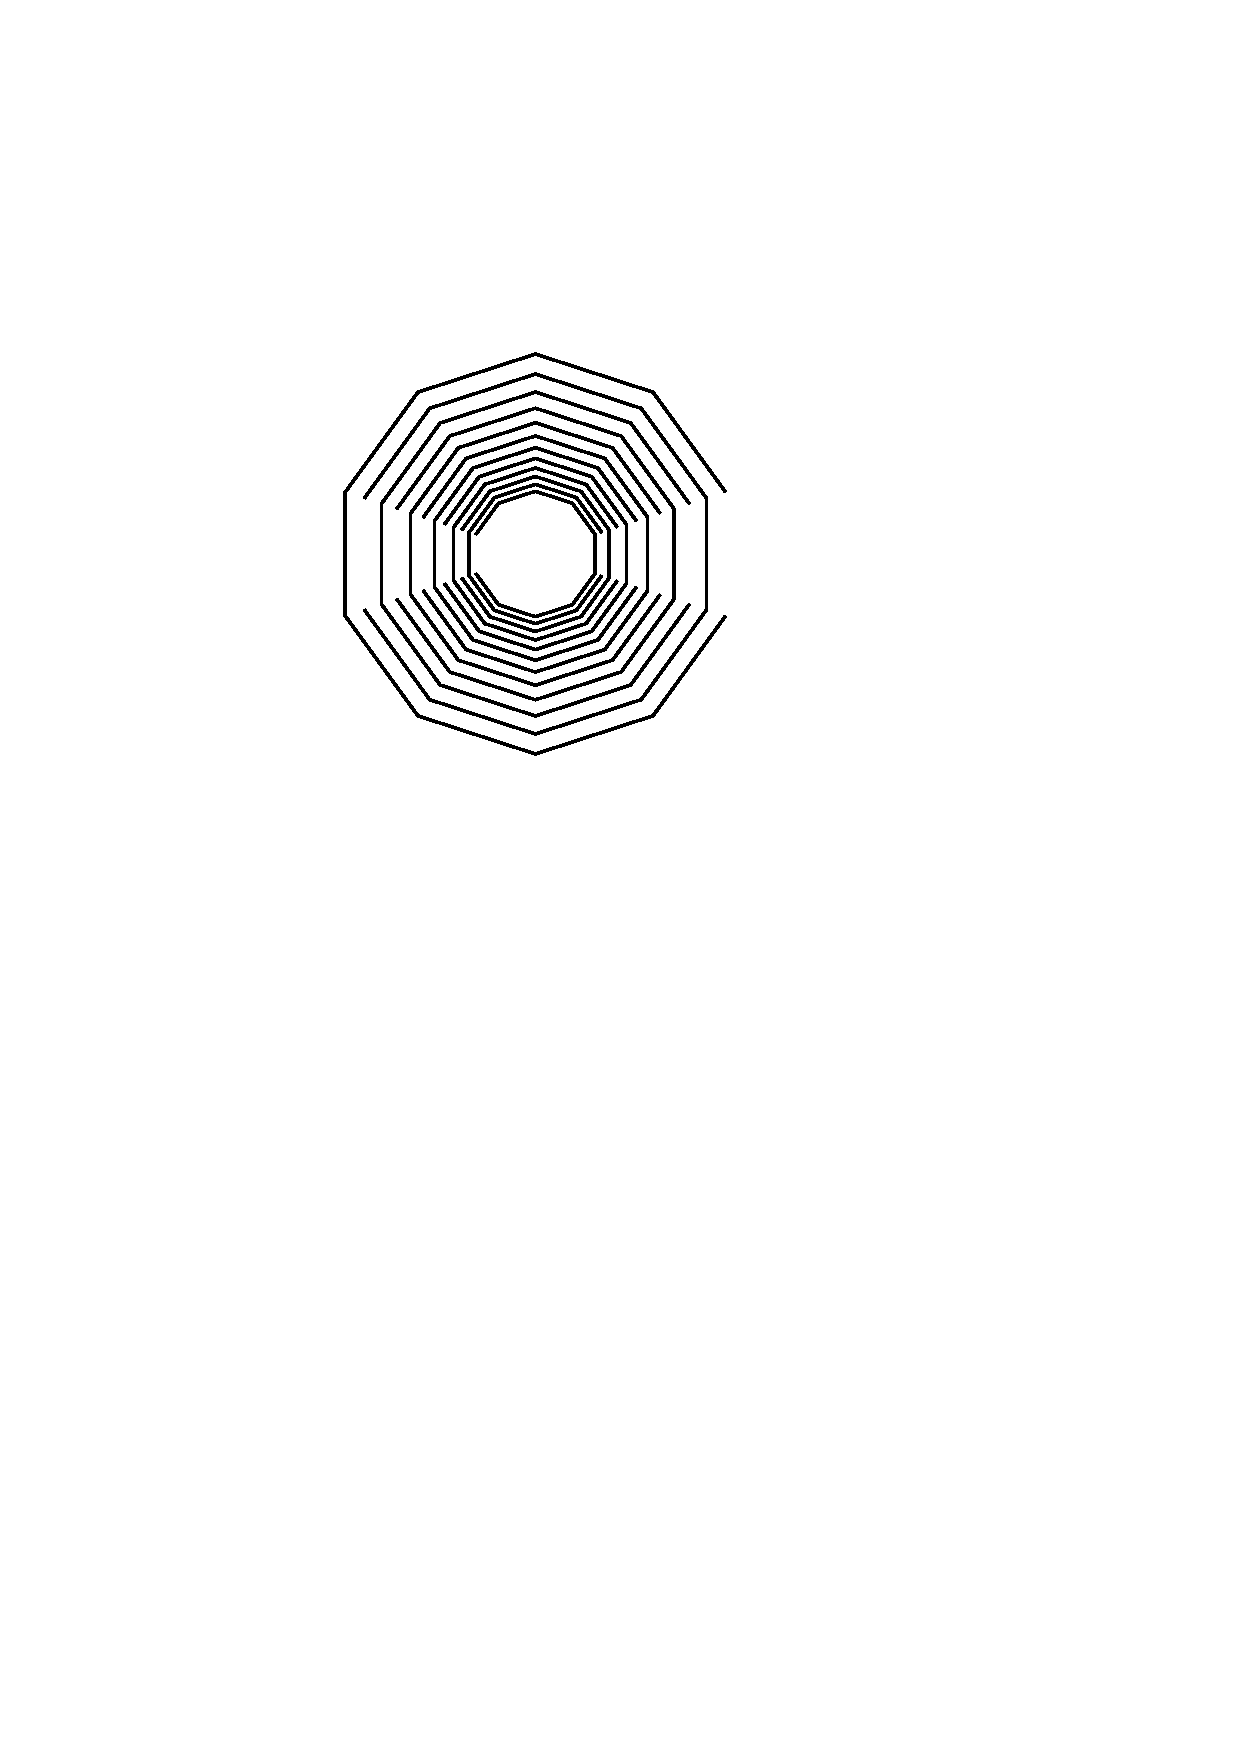
\includegraphics{lower-bound} & \includegraphics{lower-bound-b} \\
      (a) &\hspace{1cm} (b) 
      \end{tabular}
    \end{center}
    \caption{The lower-bound (a)~point set for \thmref{lower-bound}, and
      (b)~the best-case ratio $\|uw\|_G/\|uw\|$ for a pair $(u,w)$ that
      is not covered by any edge.}
    \figlabel{lower-bound}
  \end{figure}

  Let $G$ be any graph with vertex set $V$.  We say that edge a $uw$
  with $u\in A$ and $w\in B$ \emph{covers} the set of pairs
  \[
     \{ \left(u+(0,i), w+(n,j)\right) : 
          i,j\in\{-\sqrt{\alpha n},\ldots,\sqrt{\alpha n}\}\}
  \]
  for some constant $\alpha$ to be discussed later.  Thus, any edge of
  $G$ covers at most $4\alpha n$ pairs in $A\times B$.

  Next, observe that if some pair of points $u\in A$ and $w\in B$ is
  not covered by any edge of $G$, then a straightforward minimization
  argument shows that
  \[
     \frac{\|uw\|_G}{\|uw\|}
       \ge \frac{\sqrt{\alpha n}+\sqrt{(n/2)^2+(n/2-\sqrt{\alpha n})^2}}
               {n/\sqrt{2}}
       \ge \frac{\sqrt{\alpha n}+n/\sqrt{2}-O(n^{1/4})}
               {n/\sqrt{2}}
       \ge 1+\Omega(1/\sqrt{n})
  \]
  (see \figref{lower-bound}.b).
  If $G$ has $m\in O(n)$ edges, then we select $\alpha \le
  \binom{n}{2}/(8mn)$ so that
  \[  
     m4\alpha n \le \frac{\binom{n}{2}}{2} 
  \]
  In this way, at least half of the $\binom{n}{2}$ pairs of points in $V$
  are not covered by any edge and therefore,
  \[
     \asf(G) \ge 1 + \binom{n}{2}^{-1}\cdot\frac{\binom{n}{2}}{2}\cdot
          \Omega(1/\sqrt{n}) = 1 + \Omega(1/\sqrt{n}) \enspace . \qedhere
  \]
\end{proof}

We remark that the proof of \thmref{lower-bound} is easily modified to
provide a tradeoff between the number of edges of $G$ and the average
spanning ratio.  In particular, if $G$ has $m\in o(n^2)$ edges, then
\[
   \asf(G) \ge 1 + \Omega(1/\sqrt{m}) \enspace .
\]


\section*{Acknowledgement}

The authors of this paper are partly funded by NSERC and CFI.

\section*{Authors}

\paragraph{Vida Dujmovi\'c.}
School of Mathematics and Statistics and Department of Systems and Computer Engineering, Carleton University
%, \texttt{vida@cs.mcgill.ca}

\paragraph{Pat Morin and Michiel Smid.}
School of Computer Scence, Carleton University
%, \texttt{\{morin,smid\}@scs.carleton.ca}


\bibliographystyle{abbrv}
\bibliography{avgstretch}





\end{document}


